\documentclass[a4paper,12pt]{article}

\usepackage{ngerman}
\usepackage[utf8]{inputenc}
\usepackage{amsmath}
\usepackage{amssymb}
\usepackage{multicol}
\usepackage{framed}
\usepackage{graphicx}
\usepackage{hyperref}
\usepackage{array}
\usepackage{hyperref}

\usepackage[left=2.2 cm,right=2.2 cm,top=1.5cm,bottom=2.0cm]{geometry}

\newcounter{aufgnr}

\begin{document}
\begin{center}
\section*{Die Von-Neumann-Architektur}
\subsection*{Arbeitsblatt 3 - Ein grafischer Editor erleichtert das Programmieren}
\end{center}

\hrule
\vspace{.5cm}

Downloadmöglichkeiten unter \url{https://www.github.com/kur2}

\vspace{1cm}

Hinweise für die Arbeit mit dem grafischen Editor:
\begin{itemize}
\item Der Startblock gehört nicht zum Programm und wird bei der Nummerierung der Speicherzellen nicht beachtet. Er stellt den Anfangspunkt des Programmes dar und kann nicht gelöscht werden.
\item Die Ziele von Blocken, die auf Speicherzellen verweisen (z.B. alle Sprungbefehle), werden durch ziehen mit der rechten Maustaste festgelegt.
\item Das übersetzte Programm wird immer in der Datei \textit{res/progs/testProgram.txt} gespeichert
\end{itemize}


\stepcounter{aufgnr}
\subsubsection*{Aufgabe \theaufgnr: Erste Schritte:}
Gib das folgende Programm in den Editor ein, lass es übersetzen und vom Simulator simulieren:
\begin{figure}[h]
\centering
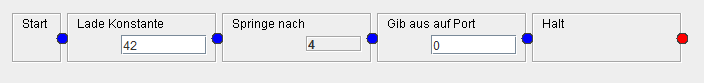
\includegraphics[scale=.65]{FirstJump.png}
\end{figure}
Was macht das Programm?\\
\\
Ändere das Programm so ab, dass statt der Zahl 42 die Zahl 64 benutzt wird.\\
\\
Ändere nun das Programm so ab, dass es den Ausgabebefehl überspringt. (Es soll kein Befehl gelöscht oder hinzugefügt werden!) Was hast du verändert und wie hast du dies getan?\\
\\
\\
\\

\stepcounter{aufgnr}
\subsubsection*{Aufgabe \theaufgnr: Manchmal springt man, manchmal nicht:}
Gib das folgende Programm in den Editor ein, lass es übersetzen und vom Simulator simulieren:
\begin{figure}[h]
\centering
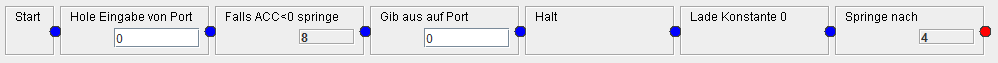
\includegraphics[scale=.47]{ConditionalJump.png}
\end{figure}
Probiere verschiedene Eingabewerte aus und beschreibe, was das Programm tut.\\
Ändere das Programm so ab, dass es den eingegebenen Wert ausgibt, falls dieser negativ ist. Ansonsten soll der Wert negativ gemacht, verdoppelt und dann ausgegeben werden. Schreibe den Programmcode in Blockschreibweise (grafischer Editor) und codiert (Zahlen in \textit{testProgram.txt}) auf.\\
\\
\\
\\


\stepcounter{aufgnr}
\subsubsection*{Aufgabe \theaufgnr: Ein Operator bleibt noch übrig - Der Modulo-Operator:}
Der Modulo-Operator gibt den Rest beim Teilen: $10 \; mod \; 3 = 1$, denn beim Teilen von 10 durch 3 bleibt 1 als Rest. $17 \; mod \; 5 = 2$, denn 17 ist $3 \cdot 5 + 2$. Schreibe ein Programm, das den Rest beim Teilen berechnet. (Wenn du nicht sicher bist, wie das geht, schau dir nochmal die ersten Programme auf dem ersten Übungsblatt an!) Berechne mit deinem Programm anschließend folgende Werte:
\begin{itemize}
\item $64~ mod~ 7 =$
\item $723~ mod~ 6 =$
\item $8947213~ mod~ 365 =$
\end{itemize}
Erweitere anschließend dein Programm so, dass die beiden Zahlen vom Benutzer eingegeben werden können. Beschreibe, was du verändert hast.\\
\\
Verändere es danach so, dass es eine 1 ausgibt, falls der Rest beim Teilen 0 ergibt. Ansonsten soll es 0 ausgeben.\\
\\
Verändere das Programm schließlich so, dass es nur eine Zahl erfragt und das Dreifache der eingegebenen Zahl ausgibt, falls sie gerade ist. Andernfalls soll das Quadrat der eingegebenen Zahl ausgegeben werden. Notiere die Programme jeweils in Blockschreibweise und codiert!\\
\\
\\
\\





\end{document}